\documentclass[]{article}

\usepackage{amsmath,amssymb}
\usepackage{tabularx,booktabs}
\usepackage{graphicx,multicol}

\usepackage{hyperref}
\hypersetup{allcolors=blue, colorlinks=true}
\usepackage[utf8]{inputenc}

% Notation
% Mathematical functions
\newcommand{\isone}[1]{{\boldsymbol{1}\left( #1 \right)}}
\renewcommand{\Pr}[1]{{\mathbb{P}\left(#1\right) }}
\newcommand{\f}[1]{{f\left(#1\right) }}
\newcommand{\Prcond}[2]{{\mbox{Pr}\left(#1\vphantom{#2}\;\right|\left.\vphantom{#1}#2\right)}}
\newcommand{\fcond}[2]{{f\left(#1|#2\right) }}
\newcommand{\Expected}[1]{{\mathbb{E}\left\{#1\right\}}}
\newcommand{\ExpectedCond}[2]{{\mathbb{E}\left\{#1\vphantom{#2}\;\right|\left.\vphantom{#1}#2\right\}}}

\newcommand{\Likelihood}[2]{\text{L}\left(#1 \left|\vphantom{#1}#2\right.\right)}
\newcommand{\sufstats}[1]{s\left(#1\right)}
\renewcommand{\exp}[1]{\mbox{exp}\left\{#1\right\}}
\newcommand{\transpose}[1]{{#1}^\mathbf{t}}

% Objects
\newcommand{\params}{\theta}
\newcommand{\Params}{\Theta}
\newcommand{\Graph}{\mathbf{G}}
\newcommand{\graph}{\mathbf{g}}
\newcommand{\GRAPH}{\mathcal{G}}
\newcommand{\Adjmat}{Y}
\newcommand{\adjmat}{y}
\newcommand{\ADJMAT}{\mathcal{Y}}

\newcommand{\INDEPVAR}{\mathcal{X}}
\newcommand{\Indepvar}{X}
\newcommand{\indepvar}{x}

\newcommand{\normconst}{\kappa\left(\params, \Indepvar\right)}

% \graphicspath{{./fig/}}


%% NEED THIS FOR CANCY TEX
\usepackage{pstricks}

% Colors
\definecolor{USCCardinal}{HTML}{990000} % 153 0 0 in RGB
\definecolor{USCGold}{HTML}{FFCC00}
\definecolor{USCGray}{HTML}{CCCCCC}

% To use the function \sout
\usepackage{ulem}
\usepackage{tabularx, booktabs}

% \bibliography{bibliography.bib}

% This avoids using underline in bibliography, why does it works? I don't know
% but just use it!
% Here is the SoF link: https://tex.stackexchange.com/questions/31566/is-it-possible-to-have-hyphenations-in-underlinedtext
\usepackage[style=numeric-comp]{biblatex}
\addbibresource{bibliography.bib}

\begin{document}
\subsection{CUG test}

CUG tests are a common way to perform hypothesis testing using social network data. Often researchers have data for a single network, and they generate a null distribution (often the U$|$MAN distribution) of a particular graph statistic by sampling networks that are similar to the network that was observed. In this applied example we have a sample of networks, therefore: (a) we have to be thoughtful about how the null is defined, and (b) we could examine the data one-graph-at-a-time, or jointly by pooling the data.

We opted for the pooled approach, because the small size of our 31 networks meant that the networks translated into a small support for the U$|$MAN distribution, (i.e., in a lot of cases the null statistic took only three unique values). The data were pooled by calculating the average count of gender-matched ties within each group. The hypothesis to test is $H_0: S^{obs} - S = 0$, where $S^{obs}$ is the observed average number of gender-matched ties and $S$ is the expected average under the assumption that gender-homophily is not a prevalent feature of the data. 

To generate the null distribution, we drew 5,000 samples and calculated the average number of gender-matched ties for each. Each sample was generated as follows: For $b = 0$ to 5,000, do:

\begin{enumerate}
    \item For each network $\graph_p$ in the data, generate a single draw from a U$|$MAN distribution conditioning on its observed dyadic census, $\graph_p^{(b)}$. This yielded a random U$|$MAN sample of 31 networks: $\left\{\graph_1^{(b)}, \dots, \graph_{31}^{(b)}\right\}$.
    \item Calculate the average number of observed gender-homophilic ties in sample $b$, using the following formula:
    \begin{equation*}
        S^{(b)} = (31)^{-1}\sum_{p=1}^{31}\sum_{(i, j) \in \graph_p^{(b)}}\adjmat_{pij}^{(b)}\isone{X_{i} = X_{j}}
    \end{equation*}
    
    Where $\adjmat_{pij}^{(b)}$ is the adjacency matrix of the $p$-th random network in the sample $b$.
    \item Next $b$.
\end{enumerate}

Ultimately, we compared the observed average of gender-matched ties, $S^{obs}$, with the generated distribution $\left\{S^{(1)}, \dots, S^{(5,000)}\right\}$. To draw graphs from the U$|$MAN distribution we used the \texttt{rguman} function included in Statnet's sna R package \cite{butts2016}. The distribution of average number of homophilic ties under the null, and the observed average, is depicted in \autoref{fig:ci-cug-null}.
 
\begin{figure}[tb]
    \centering
    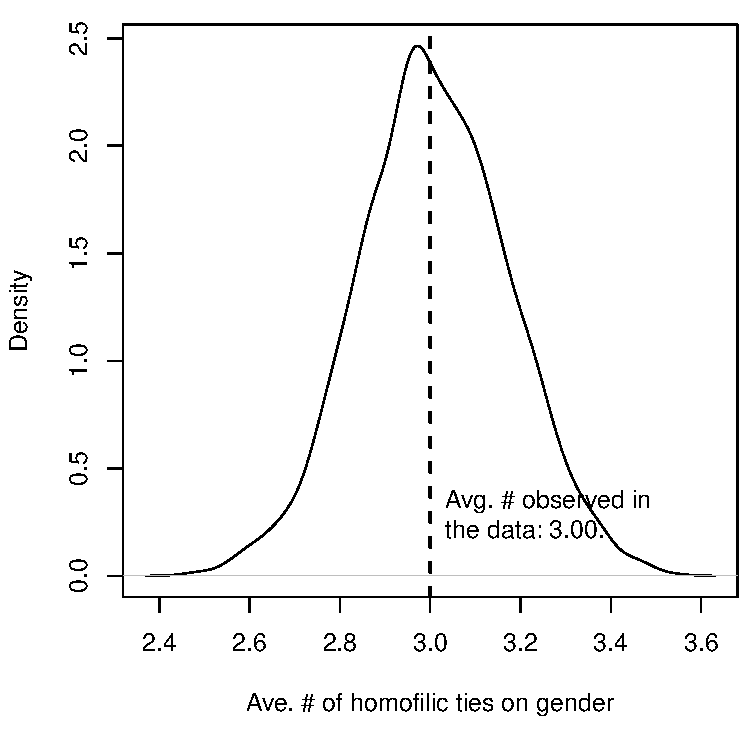
\includegraphics[width=.7\linewidth]{figures/ci-cug-test.pdf}
    \caption{Null distribution of number of average number of homophilic ties under the exact U$|$MAN distribution. The dotted line shows the location of the observed statistic $S^{obs}$.}
    \label{fig:ci-cug-null}
\end{figure}

As illustrated in figure \ref{fig:ci-cug-null}, the observed average number of gender-matched ties lies right in the middle of the null distribution; thus, failing to reject the null. Based on these results, we may conclude that gender homophily does not play a role in teammates advice seeking. While this method is useful for testing hypotheses about single processes, these uni-variate analyses are not particularly satisfying when the goal is to understand the many complex social processes that were likely to shape the networks. To do this we turn to ERGMs, which allow researchers to test more complex hypotheses and dig into social network data using a model that allows for more explicitly modeling known aspects of relational variability.
\end{document}